% ======================================================================
%  Kapitel: Training und Trainingszeit-Augmentierung
%  Gekuerzte und korrigierte Fassung
%
%  Vorausgesetzt: \code, \absatz, \px, \mAPfifty, \mAPall,
%  \zrefEpochen, \zrefBestEpoche sowie biblatex, booktabs, graphicx.
%
%  Aenderungen gegenueber der Vorfassung:
%   - "Zuweisungsgrenze" ersetzt; Kap. 3 ordnet S*sqrt(2) ausdruecklich
%     als geometrische Moeglichkeit und nicht als Detektionsgrenze ein
%   - nativer Massstab von val auf 2459 px korrigiert (war 2464; das ist
%     die auf ein Vielfaches von 32 aufgefuellte Groesse)
%   - Speicherabsatz, Optimiererliste und Gewichtsuebernahme gekuerzt
%   - patience-Begruendung und Aufloesungshinweis nur noch je einmal
%   - Zeile "Bildzwischenspeicher" aus der Budgettabelle entfernt
% ======================================================================

\chapter{Training und Trainingszeit-Augmentierung}
\label{kap:trainingszeit}

\section{Aufbau}
\label{sec:trainingsaufbau}

\absatz{Datenaufteilung.} Trainiert wird auf synthetischen Bildern, validiert
auf dem \emph{realen} \code{val}-Bild (98 Objekte). Das ist Absicht: Die
Modellauswahl muss auf der Zieldomäne erfolgen, sonst fiele die Wahl auf das
Modell, das am besten zu den eigenen Renderartefakten passt. \code{test}
(89 Objekte) berührt Training und Modellauswahl nie und dient ausschließlich der
Endbewertung. Ein vierter Split \code{sval} aus 400 synthetischen Bildern mit
anderem Seed dient allein der Messung des Sim-to-Real-Abstands
(Abschnitt~\ref{sec:simtoreal}).

\absatz{Zwei Budgets.} Die Arbeit trainiert Modelle in zwei Größenordnungen,
die nicht zu vermischen sind (Tabelle~\ref{tab:budgets}). Das
\textbf{Referenzmodell} nutzt den vollen Datensatz aus 6000 Bildern und
60~Epochen; es ist das Modell, dessen Zahlen als Ergebnis der Pipeline berichtet
werden (Abschnitt~\ref{sec:hauptergebnis}). Die \textbf{Ablationsarme} nutzen
jeweils 3000~Bilder und 30~Epochen. Dieses kleinere Budget ist eine Konzession an
die Rechenzeit -- mehrere Läufe statt einem --, und es ist \emph{für alle Arme
identisch}. Es begrenzt damit die absolute Höhe der Ablationszahlen, nicht ihren
Vergleich untereinander; Ablationszahlen sind deshalb ausschließlich mit
Ablationszahlen zu vergleichen, nie mit denen des Referenzmodells.

\begin{table}[htbp]
\centering
\caption[Die beiden Trainingsbudgets]{Die beiden Trainingsbudgets. Alles, was
nicht genannt ist, ist identisch: Architektur, Optimierer, Lernratenplan,
Verlustgewichte, Trainingszeit-Augmentierung, Seed, Validierungssplit.}
\label{tab:budgets}
\footnotesize
\begin{tabular}{@{}lcc@{}}
\toprule
 & \textbf{Referenzmodell} & \textbf{Ablationsarme (3$\times$)} \\
\midrule
Trainingsbilder & 6000 & 3000 \\
Epochenbudget & 60 (\code{patience}~20) & 30 (\code{patience}~20) \\
tatsächlich gelaufen & \zrefEpochen{} (bestes Modell: \zrefBestEpoche) & 30 \\
Batch & 8 & 8 \\
\bottomrule
\end{tabular}
\end{table}

Der Referenzlauf endete durch Early Stopping nach \zrefEpochen{} von
60~Epochen; das beste Modell stammt aus Epoche~\zrefBestEpoche. Die Batchgröße
ist nicht gewählt, sondern erzwungen: Mit Batch~16 überschritt die
$256\times256$ große P2-Merkmalskarte bei \code{imgsz}=1024 wiederholt den
freien Speicher der verwendeten Karte, und der Ausweichpfad auf die CPU macht
die Läufe von der momentanen Fremdlast abhängig und damit unvergleichbar
(Speicherwerte in Abschnitt~\ref{sec:anhangbericht}).

\absatz{Modellwahl.} Durchgängig verwendet wird \code{yolo26s-p2} mit
9,66~Millionen Parametern. Die \emph{Größe} \enquote{s} folgt aus der Datenlage:
Der Datensatz hat nur eine Klasse und neun zugrunde liegende Objektinstanzen,
die Formvielfalt und damit die nötige Modellkapazität sind also klein. Die
\enquote{nano}-Variante verliert bei 12--40\px{} großen Objekten Rückruf,
größere Varianten würden die synthetischen Eigenheiten eher auswendig lernen
\parencite{zhang2017rethinking}. Der \emph{P2-Kopf} folgt aus der
Auflösungsrechnung in Abschnitt~\ref{sec:p2kopf}. Er halbiert den Stride der
feinsten Detektionsebene von 8 auf 4 und senkt damit die kritische Größe
$S\sqrt{2}$ aus Gleichung~\eqref{eq:gridmiss} von 11,3 auf 5,7\px. Beim nativen
Maßstab liegt sie damit unter allen Objektgrößen in \code{val} und \code{test}.
Parameter kostet der P2-Kopf nicht, die \code{-p2}-Variante hat sogar 2,9\,\%
weniger als das Basismodell; teurer wird nur der Speicher.

Ausgangspunkt sind COCO-vortrainierte Gewichte. Die vortrainierten Filter der
ersten Schichten sind weitgehend domänenunabhängig \parencite{yosinski2014},
und \textcite{hinterstoisser2018} zeigen den Nutzen ausdrücklich für
synthetische Trainingsdaten. Weil die \code{-p2}-Variante über eine
Architekturdatei und nicht über einen fertigen Checkpoint definiert ist, werden
die Gewichte nur \emph{teilweise} übernommen; die zusätzlichen Blöcke der
P2-Ebene werden zufällig initialisiert.

\absatz{Modellauswahl.} Gespeichert wird der Checkpoint mit der höchsten
Fitness auf dem realen \code{val}-Bild. In der verwendeten Version~8.4.117 der
Werkzeugkette ist die Fitness allein \mAPall{} (\code{Metric.fitness} in
\code{ultralytics/utils/metrics.py}). Ältere Versionen bildeten sie als
$0{,}1\cdot\mAPfifty + 0{,}9\cdot\mAPall$; für alle Läufe dieser Arbeit führen
beide Varianten auf dieselbe beste Epoche. Diese Validierung läuft bei der
\emph{Trainings}auflösung \code{imgsz}=1024, alle berichteten Zahlen werden
dagegen beim nativen Maßstab gemessen (2459 bzw.\ 1600\px, vom Netz auf ein
Vielfaches von 32 aufgefüllt). Ausgewählt und bewertet wird also bei
unterschiedlicher Auflösung. Das ist vertretbar, weil die Rangfolge der Epochen
kaum von der Auflösung abhängt und eine zweite Validierung je Epoche viel
Rechenzeit kosten würde. Es bleibt aber eine Annahme, die für alle Läufe
gleichermaßen gilt.

\absatz{Eingabegröße.} Die Eingabegröße \code{imgsz}=1024 entspricht der
Leinwandgröße des Generators. Die synthetischen Bilder werden beim Einlesen also
\emph{nicht} skaliert, und die Objekte erreichen das Netz genau in der Größe,
für die die Pipeline ausgelegt ist (Anforderung~A2). Bei 640\px{} wären sie nach
Gleichung~\eqref{eq:deff} nur noch 7,5--27,5\px{} groß. Das untere Fünftel
dieser Spanne läge dann unter der kritischen Größe von 11,3\px{} der P3-Ebene,
die ohne P2-Kopf die feinste wäre.

\absatz{Optimierung.} Trainiert wird mit AdamW \parencite{loshchilov2019},
Startlernrate $\text{lr}_0 = 10^{-3}$ und Kosinusabfall auf 1\,\% davon
\parencite{loshchilov2017sgdr}, mit Mixed Precision \parencite{micikevicius2018},
Standard-Verlustgewichten, festem Seed und deterministischen Kerneln; die
vollständige Konfiguration steht in Tabelle~\ref{tab:trainaug} im Anhang. AdamW
ist ausdrücklich gesetzt statt \code{auto}, weil für eine Lernratensuche kein
Budget vorhanden war. Early Stopping greift nach 20 Epochen ohne Verbesserung
auf dem realen \code{val}-Bild. Das Fenster ist bewusst großzügig, weil die
Fitness an knapp hundert Objekten \emph{eines} Bildes gemessen wird und
entsprechend stark schwankt (Abschnitt~\ref{sec:trainingsverlauf}).

\section{Augmentierungsparameter zur Trainingszeit}
\label{sec:trainparam}

Auch abgeschaltete Parameter müssen begründet werden, denn einen Standardwert
auf null zu setzen ist ebenfalls eine Entscheidung.

Aktiv sind Mosaic (bei jedem Trainingsbeispiel, in den letzten zehn Epochen
abgeschaltet),
Skalierung, Translation, horizontale und vertikale Spiegelung sowie
HSV-Variation. Die Skalierung zieht einen Faktor aus $[1-a,\,1+a]$, mit
\code{scale}$\,=a=0{,}4$ also aus $[0{,}6;\,1{,}4]$; das ist etwas weniger als
die Voreinstellung $a=0{,}5$ der Werkzeugkette (Tabelle~\ref{tab:trainaug}).

Abgeschaltet sind \code{degrees}, \code{shear} und \code{perspective}. Eine
Bildrotation weitet die Boxen nach Gleichung~\eqref{eq:dbox} auf und senkt ihre
Überlappung mit der richtigen Box nach Gleichung~\eqref{eq:iou}; bei
$\theta = 10^\circ$ wird die Kantenlänge um 15,8\,\% zu groß, und die IoU sinkt
auf 0,745 (Abschnitt~\ref{subsec:aabb-rotation}). Auch \code{mixup} und
\code{cutmix} sind abgeschaltet, aber aus verschiedenen Gründen. \code{mixup}
überblendet zwei Bilder etwa im Verhältnis 1:1 und übernimmt beide Labelsätze
vollständig \parencite{zhang2018mixup}. Jedes Objekt erscheint dann
halbtransparent, trägt aber ein volles Label. \code{cutmix} setzt einen
Ausschnitt des zweiten Bildes in eine Fläche des ersten, die keine Box trifft,
und übernimmt aus dem zweiten Bild jedes Objekt, von dem mindestens 10\,\% im
Ausschnitt liegen, mit entsprechend beschnittener Box \parencite{yun2019cutmix}.
So entstehen Labels auf Objektresten bis hinab zu einem Zehntel der Fläche,
also genau das, was die Sichtbarkeitsregel des Generators mit ihrer Grenze von
30\,\% aussortiert (Abschnitt~\ref{sec:sichtbarkeit}). Selten wäre das nicht:
Auf den 6000 erzeugten Bildern findet die Werkzeugkette in 67,7\,\% der
Positivbilder eine boxfreie Fläche (\code{src/cutmix\_flaechen.py}).
\code{erasing} und \code{copy\_paste} entfallen, weil der Generator beides
physikalisch korrekt übernimmt. Die vollständige Tabelle mit Begründung je
Parameter steht im Anhang (Tabelle~\ref{tab:trainaug}).

Generator und Trainingsskalierung wirken bei der Objektgröße zusammen. Erzeugt
der Generator Objekte im Bereich $[d_{\min}, d_{\max}]$ und skaliert das
Training um einen Faktor aus $[1-a,\,1+a]$, so sieht das Netz Objektgrößen aus
\begin{equation}
  \big[\,d_{\min}\,(1-a),\;\; d_{\max}\,(1+a)\,\big].
  \label{eq:effgroesse}
\end{equation}
Mit $[d_{\min}, d_{\max}] = [12, 44]$\px{} (Gleichung~\eqref{eq:zoom},
Abschnitt~\ref{sec:modellentscheidungen}) und $a = 0{,}4$ sind das
$12 \cdot 0{,}6 = 7{,}2$ bis $44 \cdot 1{,}4 = 61{,}6$\px. Von den vier
Objekten unter 12\px, die \code{test} enthält und die der Generator selbst
nicht erzeugt (Abschnitt~\ref{sec:valtest}), sind damit drei abgedeckt; das
kleinste liegt mit 6,4\px{} knapp darunter. Nach oben reicht
die Spanne auch für stark hochskalierte Bilder. Bei sehr niedriger
Inferenzauflösung kommen die Objekte dagegen noch kleiner als 7,2\px{} im Netz
an (Abschnitt~\ref{sec:imgsz}). Die Untergrenze von 7,2\px{} liegt über der
kritischen Größe $S\sqrt{2}$ der P2-Ebene von 5,7\px{}
(Gleichung~\eqref{eq:gridmiss}), aber \emph{unter} den 11,3\px, die ohne P2-Kopf
für P3 gälten. Erst mit dem P2-Kopf erhalten also auch die kleinsten
Trainingsobjekte nach der idealisierten Rechnung aus
Abschnitt~\ref{subsec:kleine-objekte} in jeder Lage mindestens eine
Gitterposition.

\section{Trainingsverlauf}
\label{sec:trainingsverlauf}

Abbildung~\ref{abb:training} zeigt die Lernkurven der drei Ablationsarme.
Drei Beobachtungen sind unabhängig vom Ausgang der Ablation.

\emph{Erstens} fällt der Trainingsverlust über alle 30 Epochen monoton, während
die Metrik auf dem realen \code{val}-Bild deutlich früher flach wird. Das ist der
Sim-to-Real-Abstand in zeitlicher Form: Ab dem Knick verbessert das Modell
überwiegend seine Anpassung an Eigenschaften der synthetischen Daten, die in der
Zieldomäne nicht gelten. Deshalb ist es methodisch notwendig, das beste
Modell über den \emph{realen} Validierungssplit auszuwählen; eine synthetische
Validierung wählte das Modell aus der letzten Epoche und damit das am stärksten
überangepasste.

\emph{Zweitens} liegt der Trainingsverlust des Arms mit dem naiven Verdecker
(B2) unter dem der beiden anderen, obwohl alle drei exakt dieselben Objekte an
denselben Stellen enthalten. Das ist für sich genommen kein Qualitätsurteil --
ein niedriger Trainingsverlust auf synthetischen Daten sagt nichts über die
Zieldomäne --, aber es zeigt, dass der Eingriff gewirkt hat: Ein flächig grauer
Verdecker macht dieselbe Szene messbar leichter.

\emph{Drittens} verläuft die Kurve auf dem realen Bild deutlich unruhiger als der
Trainingsverlust. Das ist kein Trainingsproblem, sondern eine Folge der
Datenlage: Die Fitness wird an 98 Objekten \emph{eines} Bildes gemessen, und ein
einzelnes gefundenes oder verlorenes Objekt verschiebt den Rückruf bereits um
einen Prozentpunkt. Auf dieser Streuung beruht das großzügige
\code{patience}-Fenster aus Abschnitt~\ref{sec:trainingsaufbau}.

\begin{figure}[htbp]
\centering
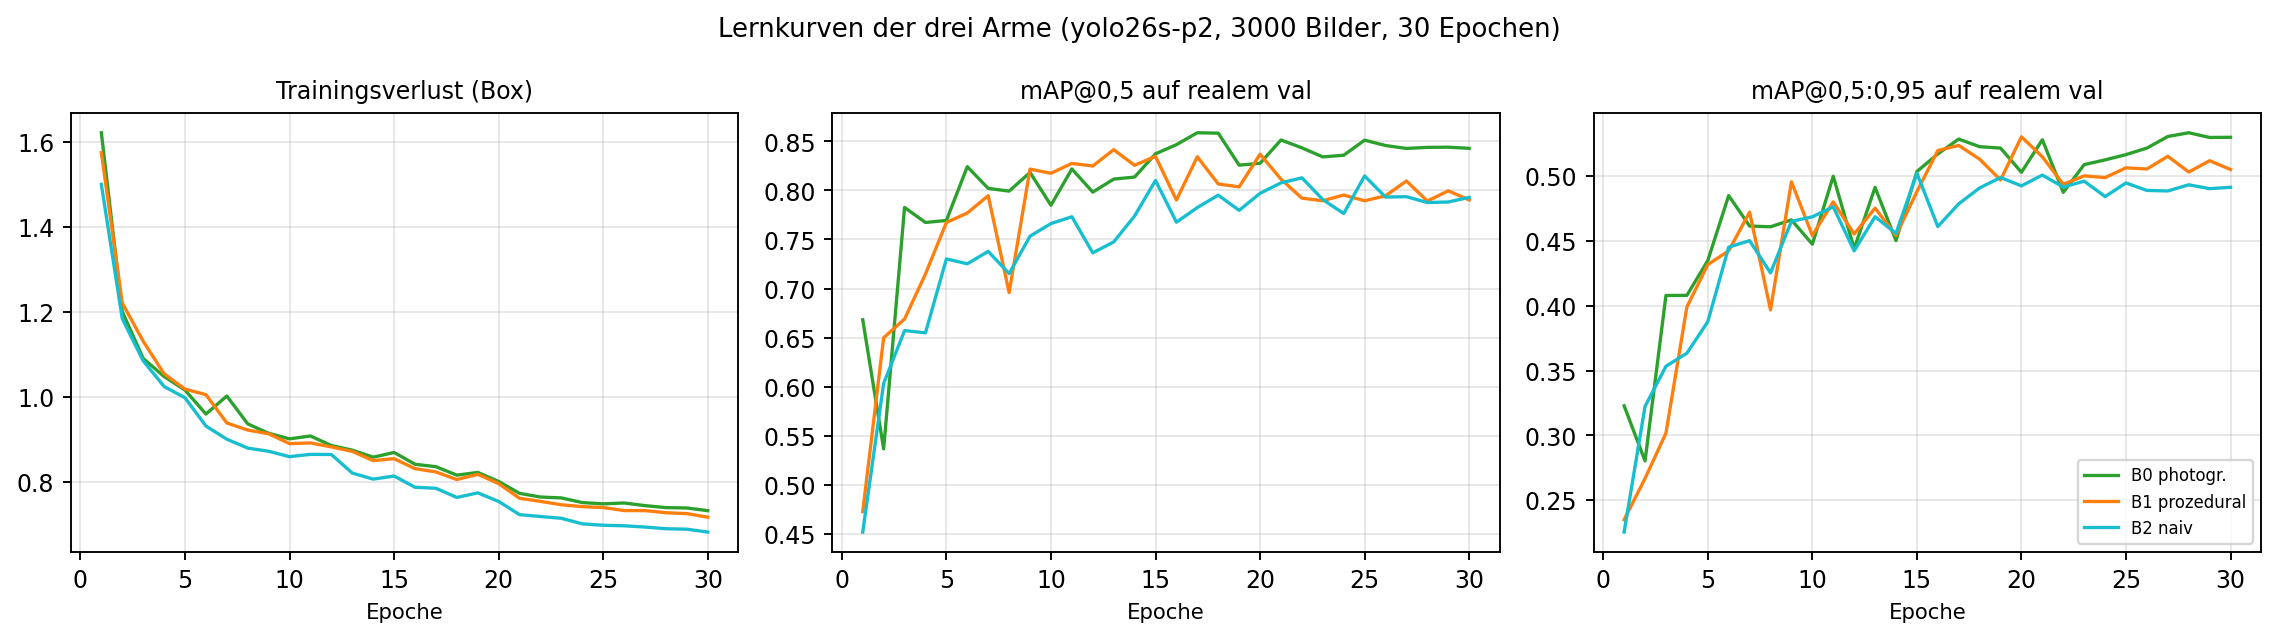
\includegraphics[width=\textwidth]{abbildungen/neu_training_b.png}
\caption[Lernkurven der Ablationsarme]{Lernkurven der drei Ablationsarme
(\code{yolo26s-p2}, 3000 Bilder, 30 Epochen, Batch~8). Links der
Box-Trainingsverlust auf den synthetischen Daten, Mitte und rechts \mAPfifty{}
und \mAPall{} auf dem realen \code{val}-Bild nach jeder Epoche -- gemessen bei
\code{imgsz}=1024 und deshalb systematisch unter den in
Kapitel~\ref{kap:auswertung} berichteten Werten. Der Knick zwischen fallendem
Verlust und flacher Realmetrik markiert den Punkt, ab dem weiteres Training
überwiegend synthetische Eigenheiten anpasst.}
\label{abb:training}
\end{figure}
